\chapter{Introduction}

\section{Background}

Complete coverage maneuvering is the task of determining and following a path such that a sensor or end-effector passes over all points of an area of interest while avoiding obstacles. This is a fundamental challenge in many robotic applications, such as lawn mowing, floor cleaning, mine detection, and environmental mapping and surveying. Determining an \emph{optimal} complete coverage path, i.e. a path that covers every point exactly once, is closely related to the well-known traveling salesperson problem, which is an NP-hard problem. %\citep{Galceran2013}
This means the computational time required to solve the problem increases drastically with the size of the input. The problem becomes even more difficult to solve in unknown and dynamic environments, where reliable information about obstacles within the area of interest is not available prior to the complete coverage task.

Thus, the need arises for online approaches that solve the problem sequentially as more and more information become available through onboard sensors. These approaches operate with no prior information about the operational area, and this relaxes the requirement of covering every point exactly once. Due to the crucial role of complete coverage maneuvering in such a wide range of applications, there are several approaches reported in the literature. Applications to robotic lawnmowers and vacuum cleaners are perhaps some of the best-known examples. For references, the reader is referred to the literature review section of this thesis.

Most research in complete coverage maneuvering is targeted towards land-based applications, while the application to marine vessels, especially online approaches, is still lacking in the literature. With new developments in sensor technologies and robotics, unmanned robots are now capable of performing many tasks that previously required manned operations. This opens up for a lot of new possibilities, and the increasing popularity of autonomous systems is prominent in many sectors. The marine sector is no exception, and it is therefore important to transfer the well-established methods of land-based robotics to marine robotics.

The Otter is a small unmanned surface vehicle (USV) designed for seabed mapping and monitoring of sheltered waters, and is equipped with a multibeam echosounder (MBES) for this purpose. The Otter is a turn-key and cost-effective solution for bathymetric surveys, and Maritime Robotics has suggested implementing complete coverage maneuvering in order to increase its autonomy. To achieve this, the USV will be equipped with a low-cost 2D lidar and other vehicle motion sensors required for collision-free maneuvering on the water surface. The Otter will simultaneously keep track of obstacles on the surface with the lidar, and the covered area of the seabed with the multibeam echosounder. With this information, the USV will generate and follow collision-free paths on the surface in order to achieve complete coverage of the seabed. The Otter USV and an illustration of a bathymetric survey are shown in \figref{fig:background}.

\begin{figure}[h!]
    \centering
	\makebox[\linewidth][c]{
	\begin{subfigure}[b]{0.5\textwidth}
		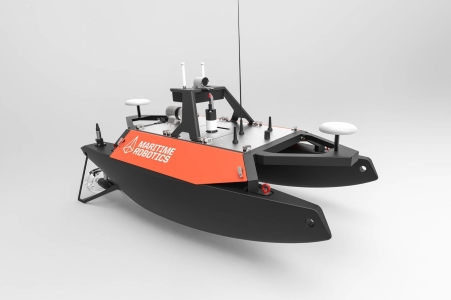
\includegraphics[width=1\linewidth]{fig/intro/otter_cgi}
		\caption{}
		\label{fig:otter}
	\end{subfigure}
	\begin{subfigure}[b]{0.5\textwidth}
		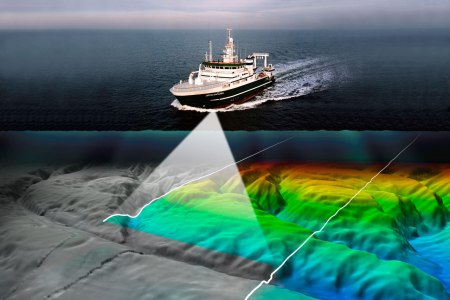
\includegraphics[width=1\linewidth]{fig/intro/seabed_mapping}
		\caption{}
		\label{fig:seabed_mapping}
	\end{subfigure}
	}
	\caption[The Otter USV and seabed mapping.]{(a) The Otter USV, courtesy of Maritime Robotics. (b) A surface vessel mapping the seabed with a multibeam echosounder, courtesy of the Marine Institute.} \label{fig:background}
\end{figure}

\section{Objective}

The main objective of this thesis is the following:

\begin{itemize}[label=\ding{212}]

\item Design, implement and test a complete coverage maneuvering system for the Otter USV using a low-cost lidar.

\end{itemize}

\noindent The system should be capable of carrying out bathymetric surveys in unknown environments without operator assistance. Based on this main objective, there are 3 subobjectives:

\begin{itemize}[label=\ding{213}]

\item Autonomous operation requires accurate real-time information about the USV and its immediate surroundings. Data from several sensors must be fused in order to accurately localize the USV. In addition, a sufficiently detailed map of the surroundings has to be provided for use in path planning.

\item A complete coverage path planning (CCPP) method must be implemented. The method should be able to generate a collision-free feasible path that ensures coverage of the desired survey area. Furthermore, this path needs to be generated online from available sensor data.

\item A guidance and path following method must be implemented. The USV must be able to follow the path generated from the complete coverage path planning method.

\end{itemize}

\noindent In order to accomplish these objectives, the author has, together with the supervisors, formulated the work description attached in the MSc thesis description in the beginning of this thesis.

\section{Thesis contributions}

The main contributions of this thesis are:

\begin{itemize}

\item A simulator for the Otter USV has been developed for ROS Melodic and Gazebo 9. The simulator implements low-level controllers and is capable of providing simulated input from several sensors, including GNSS, IMU and lidar. The simulator has been thoroughly tested and can be used for verification of methods and algorithms, including methods for SLAM, sensor fusion, path planning, guidance and path following.

\item A strategy for sensor fusion and simultaneous localization and mapping (SLAM) with Cartographer. The implemented system fuses data from GNSS, IMU and 2D lidar to provide localization and mapping of the surrounding environment.

\item A map processing strategy and two methods for partitioning of the operational workspace. One of them is particularly suited for variable coverage range sensors.

\item Two online CCPP methods. Obstacle avoidance is performed in both methods using a 2D lidar. One of the methods applies a variable inter-lap spacing, which to the author's knowledge has not yet been done in an online CCPP method for seabed mapping with obstacle avoidance. 

\item A method that ensures feasibility of the generated path regarding the Otter USV's turning radius and speed.

\item A path following method for the USV that can track the generated path.

\item An interface to Maritime Robotics' onboard system on the Otter USV for controlling the USV's thrusters from ROS.

\end{itemize}

\noindent All implementations are written in C++ for ROS Melodic and are available in the electronic attachment of this thesis, as well as on the author's GitHub page: \url{https://github.com/jhlenes/complete_coverage} and \url{https://github.com/jhlenes/usv_simulator}. These code repositories provide a good starting point and reference for further work with the Otter USV or other development in ROS.

\section{Scope and limitations}

%\todo[inline]{Scope and delimitations that emerge from the research question and objectives must be clearly explained in a separate section.}

\subsection{Outline}

The thesis is organized as follows:\vspace{0.4em}

\noindent \textbf{Chapter 2:} Provides background information and literature references on relevant topics and theory. This includes the Otter USV and its sensor package, workspace partitioning, relevant CCPP methods, and feasible path design. 
\vspace{0.4em}

\noindent \textbf{Chapter 3:} Presents the problem formulation which further defines the problem to be solved. The problem is broken down and formulated as several subproblems that can be solved individually.
\vspace{0.4em}

\noindent \textbf{Chapter 4:} Describes which sensors are necessary, how sensor data is gathered and how it is fused together with data from other sensors. The SLAM system Cartographer is introduced.
\vspace{0.4em}

\noindent \textbf{Chapter 5:} Presents how the SLAM map is processed and partitioned to represent the workspace in a way suitable for CCPP.
\vspace{0.4em}

\noindent \textbf{Chapter 6:} Describes in detail how the CCPP methods work. This includes how the underlying workspace representation is used, which strategies to use in the path planning, how to ensure complete coverage, and how to generate the waypoints.
\vspace{0.4em}

\noindent \textbf{Chapter 7:} Presents how feasible paths are generated from waypoints. A line-of-sight (LOS) guidance law for curved paths that generates continuous steering control capable of tracking these paths is also covered.
\vspace{0.4em}

\noindent \textbf{Chapter 8:} Presents results of simulations with sensor fusion and SLAM, CCPP and path following. The results are discussed with regards to reliability and performance.
\vspace{0.4em}

\noindent \textbf{Chapter 9:} Presents results of real-world experiments with the Otter USV in the harbor of Trondheim. The results are discussed with regards to reliability and performance.
\vspace{0.4em}

\noindent \textbf{Chapter 10:} Presents concluding remarks regarding the implemented system. Recommendations and suggestions for further work are also presented.
\vspace{0.4em}

\subsection{Limitations}

Some of the limitations of the implemented system are:

\begin{itemize}

\item No distinction is made between moving and stationary obstacles. This may result in some undesirable behavior regarding moving obstacles. The system is not in compliance with the Convention on the International Regulations for Preventing Collisions at Sea (COLREGs).

\item The system is only tested in simulations and experimentally in a harbor. Different environments might offer other challenges not accounted for.

\item The system has not been tested experimentally with a multibeam echosounder. Varying depth is only considered in simulations.

\item The Otter USV already has low-level control developed by Maritime Robotics. Thus, the implemented system will restrict itself to high-level planning and provide course and speed control as input to the existing onboard system.

\item A low-cost 2D lidar is the only range-based sensor, obstacles outside the lidar's scan plane are not detected.

\end{itemize}

